\documentclass[11pt,oneside]{article}
\newcommand{\R}{\mathbb{R}}
\newcommand{\C}{\mathbb{C}}
\newcommand{\Z}{\mathbb{Z}}
\newcommand{\N}{\mathbb{N}}
\usepackage[french]{babel}
\usepackage[utf8]{inputenc}
\usepackage[T1]{fontenc}
\usepackage{lmodern}
\usepackage{array}
\usepackage{multicol}
\usepackage{titlesec}
\usepackage{graphicx}
\usepackage[margin=3cm]{geometry}
% \usepackage{fullpage}
% \usepackage{common}
\usepackage{amsmath,amsfonts,amssymb}
% \usepackage{overpic,boxedminipage}
\usepackage{hyperref}
\DeclareMathOperator*{\argmin}{arg\,min}
\DeclareMathOperator{\cotan}{cotan}
\DeclareMathOperator{\sinc}{sinc}
\DeclareMathOperator{\Tr}{Tr}
\DeclareMathOperator{\tr}{tr}
\DeclareMathOperator{\Gram}{Gram}
\DeclareMathOperator{\diag}{diag}
\newcommand{\lp}{\left(}
  \newcommand{\rp}{\right)}
\usepackage{blkarray}
\usepackage{multirow}
\usepackage{framed,fancybox}
\usepackage{tikz}
% \usepackage{algorithm2e}
% \usepackage{algorithmic}
\usepackage{float}
\usepackage{framed}
% \usepackage{ulem}
\usetikzlibrary{shapes,arrows}

\newcommand{\lela}{\left \langle}
  \newcommand{\rira}{\right \rangle}
\newcommand{\norm}[1]{\left\lVert#1\right\rVert}
\newcommand{\abs}[1]{\left|#1\right|}
\newtheorem{remarque}{Remarque}

\title{iXBlue}
\author{}
\date{}
\begin{document}
\maketitle
% \setcounter{secnumdepth}{1}
\setcounter{tocdepth}{1}
\tableofcontents

\section{Introduction}
\section{Recalage}
\section{Optimisation de trajectoire}
\subsection{Deuxième algorithme de Dijkstra}
\subsubsection{Sélection de points}
\begin{figure}[hbtp]
\begin{center}
\begin{tikzpicture}[scale=0.5]
\draw[gray] (0,0) grid[xstep=0.125,ystep=0.125] (1,1);
\draw (0,0) grid (8,8);
\draw[->,>=latex] (-0.35,0.3) -- (0.2,0.3);
\draw node[left] at (-0.25,0.3) {$C$};
\end{tikzpicture}
\end{center}
\caption{Partitionnement de la carte de la bathymétrie}
\end{figure}

On propose un algorithme qui permet de sélectionner une partie des points de la carte qu'on considère intéressants. Réduire le nombre de noeuds du graphe est important car cela permet de réduire le coût de calcul de l'algorithme de Dijkstra. L'idée est que le recalage est a priori plus efficace lorsque la variation de la bathymétrie est importante autour du point où l'on effectue la mesure. Cet algorithme se décompose en quatre étapes
\begin{enumerate}
\item On effectue un partitionnement de la carte de bathymétrie.
\item On choisit un seuil $r\in (0,1)$.
\item Dans chaque sous partie $C$ , on sélectionne l'ensemble des points $P$ tels que $\|\nabla h(P)\|\geq \|\nabla h\|_{\mathit{L}^\infty(C)}(1-r)$.
\item On rajoute les points de départ et d'arrivée s'ils n'ont pas été sélection dans l'étape 3.
\end{enumerate} 
\begin{remarque}
Dans le cas où la bathymétrie est constante dans chacune des sous parties, l'algorithme sélectionne tous les points de la carte.
\end{remarque}
\begin{remarque}
Suivant le partitionnement de la carte et la valeur du seuil $r$, il n'est a priori pas garanti que le graphe puisse relier le point de départ et le point d'arrivée. Il faut rajouter des conditions sur la manière de partitionner et/ou le seuil qui seront à déterminer.
\end{remarque}

\subsubsection{Définition du coût}
Soient $P$ un noeud du graphe et $Q\in E_P$, on définit le coût associé à l'arète qui relie les deux points par
\begin{align*}
c(P,Q)=c(\{P,Q\}) \text{ pour tout }Q\in E_P.
\end{align*}
\subsection{Résultats}
Cette section présente les résultats des trois méthodes d'optimisation pour différents types de bathymétrie.

Le coût (le long de la trajectoire) de la trajectoire obtenue par l'algorithme glouton est plus grand que ceux obtenues avec les algorithmes de Dijkstra dans les différents cas considérés. L'approche globale de l'algorithme de Dijkstra est plus performante que la stratégie locale de l'algorithme glouton sur ce problème.

\subsubsection{Bathymétrie uniforme}
On considère la bathymétrie
\begin{align*}
h(x,y)=h_0.
\end{align*}
Cette carte de bathymétrie correspond au cas où le recalage ne nous donnerai pas d'information pour réduire la zone d'incertitude. Les résultats sont présentés dans la table \ref{tab_const}. 

\begin{table}
\begin{tabular}{cc}
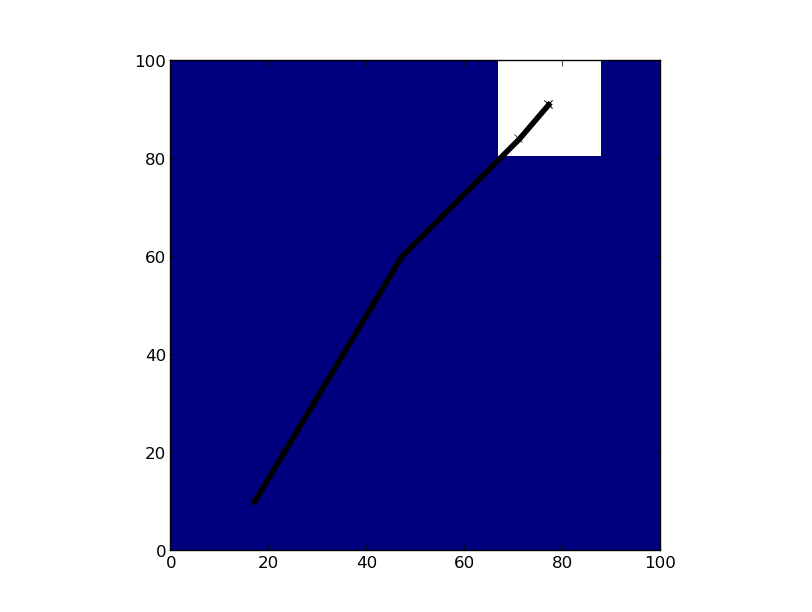
\includegraphics[scale=0.42]{../data/greedy_const/plot_A_10_17_B_91_77_iteration_010.png} &
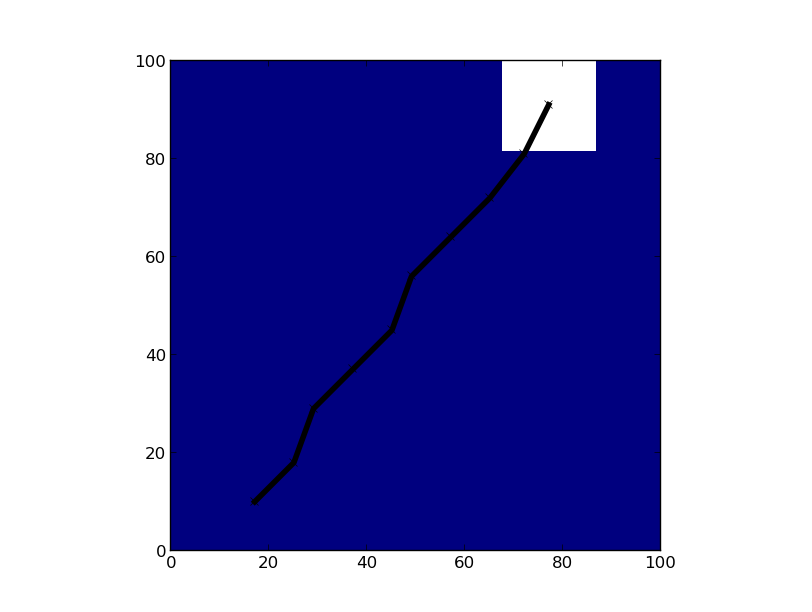
\includegraphics[scale=0.42]{../data/anneaux_const/plot_A_10_17_B_91_77_iteration_009.png} \\
Glouton, coût = 1749&Dijkstra 1, coût = 1329\\
&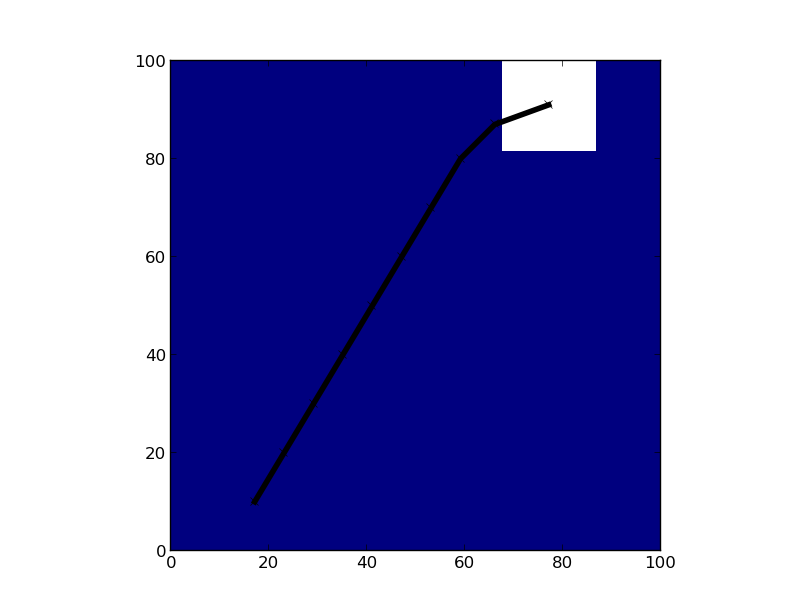
\includegraphics[scale=0.42]{../data/gradient_dijkstra_const/plot_A_10_17_B_91_77_iteration_009.png} \\
&Dijkstra 2, coût = 1329\\
\end{tabular}
\caption{Trajectoires, incertitudes à l'instant final et coût le long de la trajectoire}
\label{tab_const}
\end{table}
\subsubsection{Bathymétrie plane}
On considère la bathymétrie
\begin{align*}
h(x,y)=h_0 + \alpha y.
\end{align*}
 Les résultats sont présentés dans la table \ref{tab_plane}.
\begin{table}
\begin{tabular}{cc}
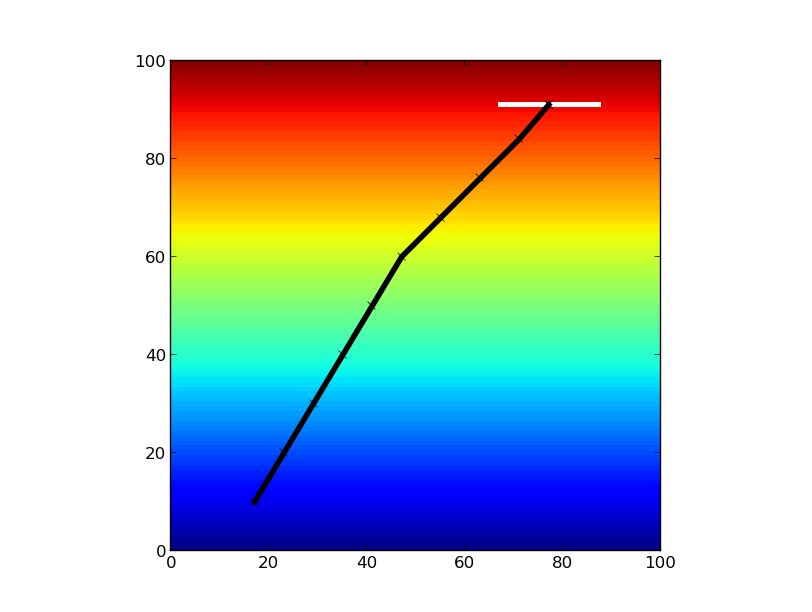
\includegraphics[scale=0.42]{../data/greedy_plane_2/plot_A_10_17_B_91_77_iteration_010.png} &
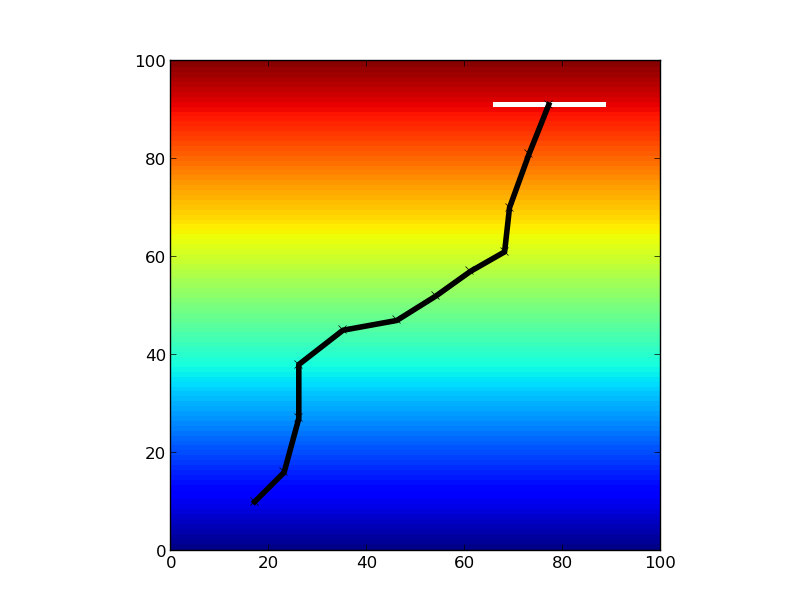
\includegraphics[scale=0.42]{../data/anneaux_plane_2/plot_A_10_17_B_91_77_iteration_011.png} \\
Glouton, coût = 120 &Dijkstra 1, coût = 69 \\
&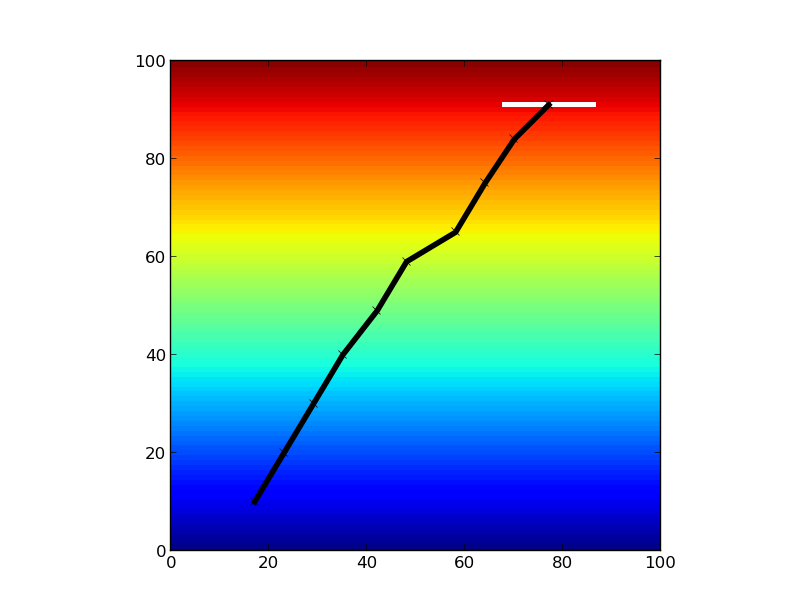
\includegraphics[scale=0.42]{../data/gradient_dijkstra_plane_2/plot_A_10_17_B_91_77_iteration_009.png} \\
&Dijkstra 2, coût = 99\\
\end{tabular}
\caption{Trajectoires, incertitudes à l'instant final, et coût le long de la trajectoire}
\label{tab_plane}
\end{table}
\subsubsection{Bathymétrie avec symétrie sphérique}
On considère la bathymétrie
\begin{align*}
h(x,y)=h_0-\alpha (x^2+y^2).
\end{align*}
 Les résultats sont présentés dans la table \ref{tab_cone}.
\begin{table}
\begin{tabular}{cc}
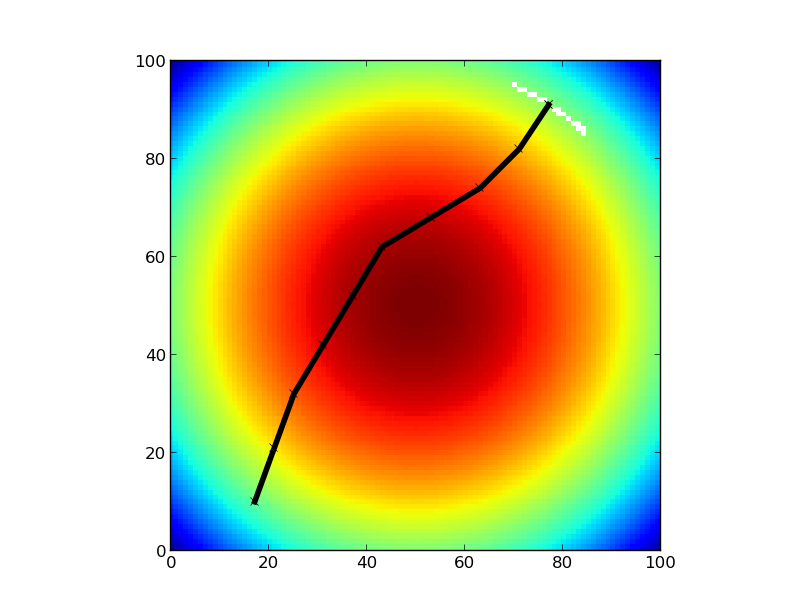
\includegraphics[scale=0.42]{../data/greedy_cone_2/plot_A_10_17_B_91_77_iteration_010.png} &
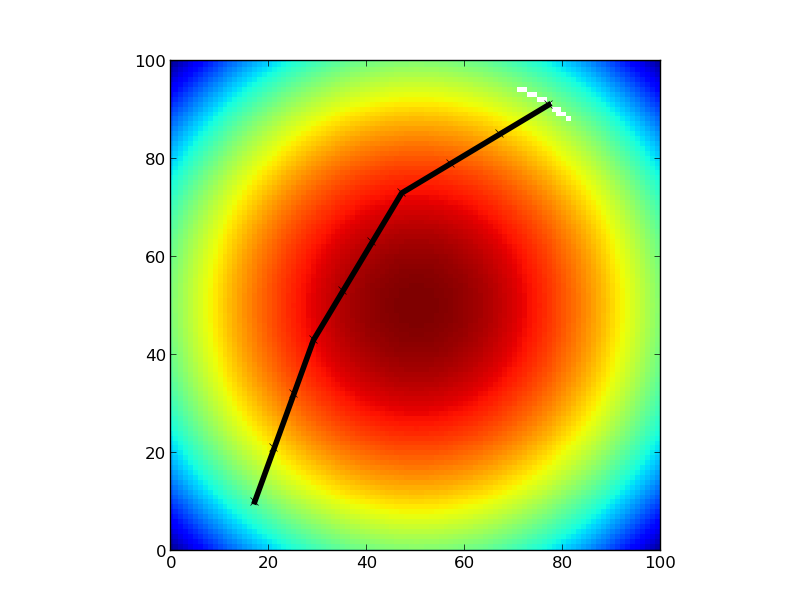
\includegraphics[scale=0.42]{../data/anneaux_cone_2/plot_A_10_17_B_91_77_iteration_009.png} \\
Glouton, coût = 178&Dijkstra 1, coût = 143\\
&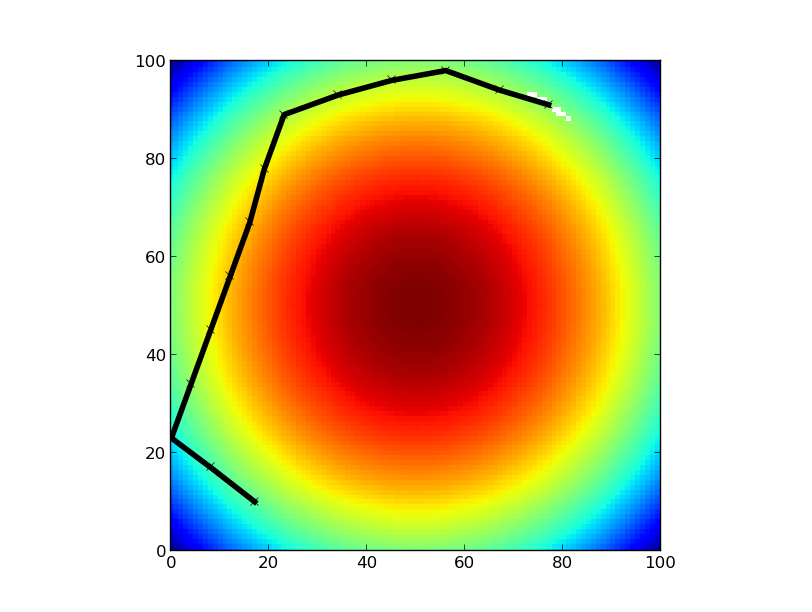
\includegraphics[scale=0.42]{../data/gradient_dijkstra_cone_2/plot_A_10_17_B_91_77_iteration_013.png} \\
&Dijkstra 2, coût = 129\\
\end{tabular}
\caption{Trajectoires, incertitudes à l'instant final et coût le long de la trajectoire}
\label{tab_cone}
\end{table}
\subsubsection{Bathymétrie de la morne rouge}
On considère la bathymétrie de la morne rouge. Les résultats sont présentés dans la table \ref{tab_morne}.
\begin{table}
\begin{tabular}{cc}
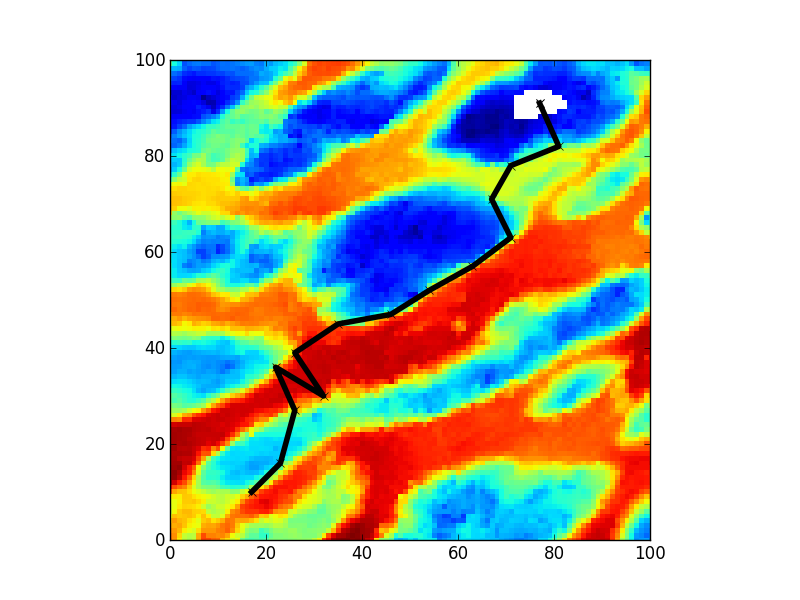
\includegraphics[scale=0.42]{../data/greedy/plot_A_10_17_B_91_77_iteration_015.png} &
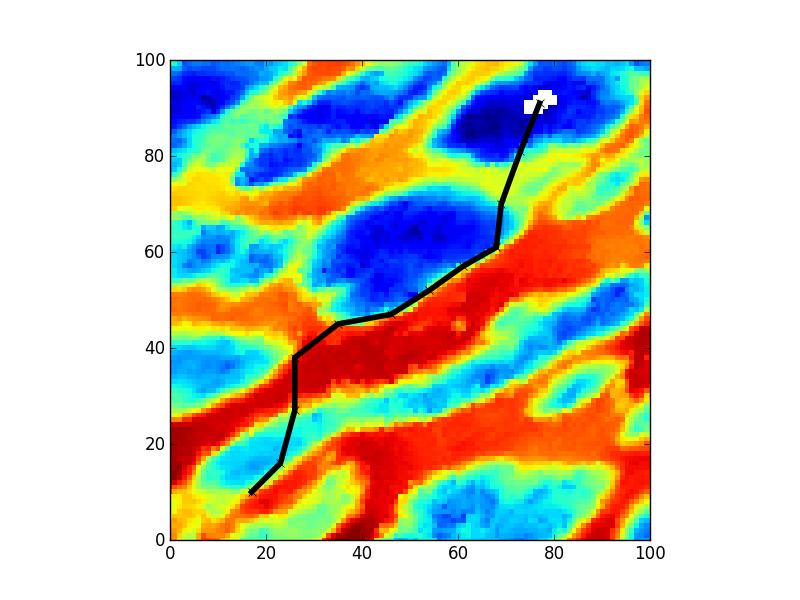
\includegraphics[scale=0.42]{../data/anneaux/plot_A_10_17_B_91_77_iteration_011.png} \\
Glouton, coût = 147&Dijkstra 1, coût = 69\\
&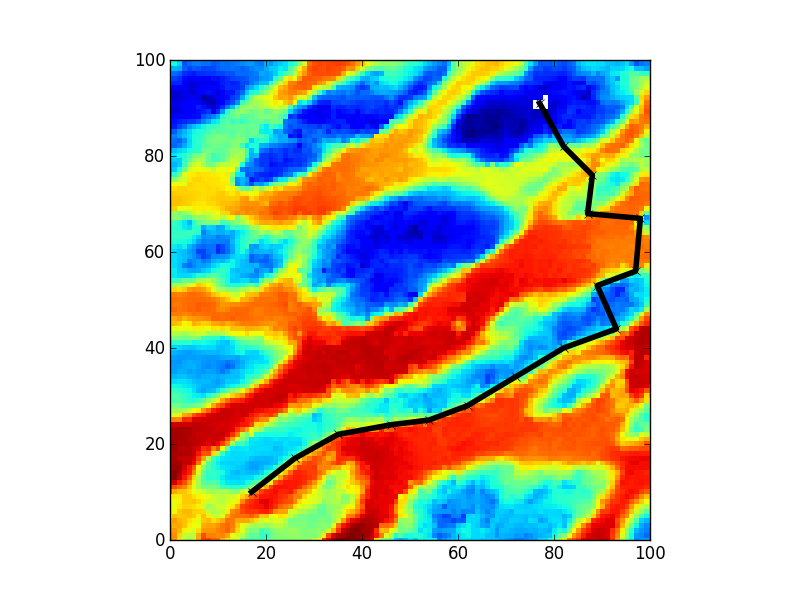
\includegraphics[scale=0.42]{../data/gradient_dijkstra/plot_A_10_17_B_91_77_iteration_015.png} \\
&Dijkstra 2, coût = 97\\
\end{tabular}
\caption{Trajectoires et incertitudes à l'instant final et coût le long de la trajectoire}
\label{tab_morne}
\end{table}


\section{Pistes continues}
\paragraph{Modèle jouet}
  On cherche à aller sur des zones de grande pente:
  \begin{align*}
    c(\gamma) = -\int_{t=0}^{1} |\nabla h(\gamma(t))|^{2}  dt
  \end{align*}

  Mal posé (les suites minimisantes se localisent sur les maxima de
  $\nabla h$) : régularisation~?
  
\begin{align*}
  c(\gamma) =  \int_{t=0}^{1} a |\gamma'(t)|^{2} - b |\nabla
  h(\gamma(t))|^{2} dt
\end{align*}

Bien posé~? Minimiseurs~? Comment prendre en compte l'heuristique que
$\gamma$ doit alterner les directions de $\nabla h$ pour se localiser~?

% \begin{align*}
%   c(\gamma) =  \int_{t=0}^{1} a |\gamma'(t)|^{2} - b |\nabla
%   h(\gamma(t)) \cdot \gamma'(t)| dt
% \end{align*}

\paragraph{Un modèle un peu plus complexe}
Modèle effectif pour les incertitudes en $x$ et $y$ $\sigma_{x}$ et
$\sigma_{y}$ :
\begin{align*}
  c(\gamma) &= \sigma_{x}(1) + \sigma_{y}(1), \text{ où}\\
  \dot \sigma_{x} &= a - b \sigma_{x} (\partial_{x} h(\gamma(t)))^{2}\\
  \dot \sigma_{y} &= a - b \sigma_{y} (\partial_{y} h(\gamma(t)))^{2}.
\end{align*}
Amortissement exponentiel vers un point d'équilibre $\sigma_{x} \sim
1/(\partial_{y} h(\gamma(t)))^{2}$. Sous la forme générale d'un
contrôle optimal. Problème : modèle non isotrope (trajectoires
diagonales~?)

Généralisation : représenter l'incertitude par une matrice SDP $A$. Si
on pose $G = \nabla h \nabla h^{T}$,
\begin{align*}
  \dot A = a A - b \sqrt G A \sqrt G.
\end{align*}
On modifie les incertitudes dans la direction $\nabla h$, on n'y
touche pas dans $\nabla h^{\perp}$. Problème : $A$ ne reste
pas forcément SDP. Y a-t-il une bonne généralisation~?

\section{Pistes probabilistes}
  \paragraph{Modélisation des incertitudes}
\begin{itemize}
\item Sources d'incertitude : précision de l'accéléromètre, erreurs
  d'intégration (fréquence finie), erreur numérique (stockage en
  virgule flottante)
\item Dérive de l'estimation de position
\item Modélisation délicate
\item Si on fait une erreur initiale sur l'accélération, dérive en
  $t^{2}$
\item Si on fait une erreur initiale sur la vitesse, dérive en
  $t$
\item Compensation des erreurs~? Marche aléatoire, dérive en $\sqrt t$
 ~? $t^{3/2}$~? $t^{5/2}$~?
\item Non trivial en pratique
\end{itemize}
\paragraph{Modélisation probabiliste}
  \begin{itemize}
  \item Une approche par intervalles néglige la compensation des erreurs
    et est trop pessimiste. Modèle probabiliste~?
  \item Soit $(x_{0}, x_{1} \dots, x_{N})$ le chemin suivi par le
    sous-marin, supposé exact.
  \item Soit $X_{n}$ la position estimée du sous-marin. Loi de
    $X_{n+1}$~?
  \item Sans bathymétrie, on met à jour la position avec le vecteur
    vitesse $v_{n} = x_{n+1} - x_{n}$, entaché (pour simplifier) d'une erreur aléatoire
    $\varepsilon_{v} \sim N(0, \sigma_{v})$
  \item La bathymétrie nous donne $h(X_{n+1}) = h(x_{n+1}) +
    \varepsilon_{h}$, avec une erreur $\varepsilon_{h} \sim N(0, \sigma_{h})$
  \end{itemize}

  \begin{center}
  \boxed{\mbox{$X_{n+1} \sim L(X_{n} + v_{n} + \varepsilon_{v} \;\Big|\;
    h(X_{n} + v_{n} + \varepsilon_{v}) = h(x_{n+1}) + \varepsilon_{h})$}}
  \end{center}
  \begin{center}
  \boxed{\mbox{$X_{n+1} \sim L(X_{n} + v_{n} + \varepsilon_{v} \;\Big|\;
    h(X_{n} + v_{n} + \varepsilon_{v}) = h(x_{n+1}) +  \varepsilon_{h})$}}
  \end{center}

  En notant formellement $P(X=x)$ pour la densité de $X$ en $x$,
  \begin{align*}
    P(X_{n+1} = x) &= P(X_{n} + v_{n} + \varepsilon_{v} = x \;\Big|\;
    h(X_{n} + v_{n} + \varepsilon_{v}) = h(x_{n+1}) + 
                     \varepsilon_{h})\\
    &= \frac 1 N P(X_{n} + v_{n} + \varepsilon_{v} = x \cap
    h(X_{n} + v_{n} + \varepsilon_{v}) = h(x_{n+1}) + \varepsilon_{h})\\
    &= \frac 1 N P(X_{n} + v_{n} + \varepsilon_{v} = x) \; P(h(x) = h(x_{n+1}) + \varepsilon_{h}),
  \end{align*}
  où $N$ est choisi pour normaliser $X_{n+1}$.

  On calcule $P(h(x) = h(x_{n+1}) + \varepsilon_{h})$ (facile si
  $\varepsilon_{h}$ est gaussienne), on calcule $P(X_{n} + v_{n} +
  \varepsilon_{v} = x)$ (translation et convolution), on multiplie et on
  normalise. En théorie bien plus précis que l'approche par boites,
  mais quel traitement des incertitudes de vitesse~? Lien avec les
  filtres de Kalman~?
\section{Conclusion}
\section{Bibliographie}
\end{document}
